\documentclass[11pt,a4paper]{article}
\usepackage[margin=2.2cm]{geometry}
\usepackage{amsmath,amssymb}
\usepackage{booktabs}
\usepackage{listings}
\usepackage{xcolor}
\usepackage{hyperref}
\usepackage{tikz}
\usetikzlibrary{positioning,arrows.meta,calc}

\lstset{
  basicstyle=\ttfamily\small,
  keywordstyle=\color{blue!70!black}\bfseries,
  commentstyle=\color{gray},
  stringstyle=\color{orange!70!black},
  numbers=left, numberstyle=\tiny\color{gray},
  frame=single, breaklines=true, columns=fullflexible,
  showstringspaces=false, language=Python,
}

\title{\textbf{CubeMars AK60-6 V3.0 KV80}\\[2pt]
       \large Internal notes -- MIT protocol, wiring, calibration,\\
       servo-mode vs.\ MIT-mode, troubleshooting}
\author{Repo \texttt{exo-actuator-sensor-drivers}}
\date{\today}

\begin{document}\maketitle
\tableofcontents
\newpage

% =========================================================================
\section{What it is}
\label{sec:intro}
% =========================================================================

The \textbf{CubeMars AK80-9 KV60} is a brushless servo motor with an
integrated planetary gearbox and dual magnetic encoders, designed for
force-torque controlled robotic joints.  It uses the same
\textbf{MIT mini-cheetah CAN protocol} (hereafter \emph{MIT mode}) that
was published by the MIT Biomimetic Robotics Lab for their
mini-cheetah actuators and subsequently adopted by many vendors
(CubeMars, T-Motor, Damiao, and others).

\begin{center}\small
\begin{tabular}{ll}
\toprule
Property & Value \\
\midrule
Model              & AK60-6 V3.0 KV80 \\
Voltage            & 18--52\,V (rated 48\,V) \\
Rated current      & 10\,A \\
Peak current       & 30\,A \\
Gear ratio         & 6:1 planetary \\
Output torque (cont.) & $\approx$5\,N$\cdot$m \\
Output torque (peak)  & 15\,N$\cdot$m \\
Output speed (no-load)& $\approx$45\,rad/s at 48\,V \\
Position range     & $\pm 12.5$\,rad (firmware MIT limit, \texttt{PMAX}) \\
Encoder            & dual 14-bit magnetic (rotor + output shaft) \\
CAN bus            & 1\,Mbps standard or extended frame \\
CAN mode (our driver) & \textbf{MIT mode only} (see Section~\ref{sec:modes}) \\
CAN ID (bench)     & \textbf{0x68 = 104} (confirmed via scan 12~May~2026) \\
R-Link MIT setting & \textbf{Inquiry Feedback} (not ``Periodic Feedback'') \\
Configuration tool & R-Link (CubeMars Windows application) \\
\bottomrule
\end{tabular}
\end{center}

% =========================================================================
\section{What is the ``MIT CAN protocol''?}
\label{sec:mit}
% =========================================================================

\subsection{Background}

The MIT mini-cheetah actuator protocol was developed at MIT's
Biomimetic Robotics Lab and first described in:

\begin{quote}
  Ben Katz, \textit{A Low Cost Modular Actuator for Dynamic Robots},
  M.Eng.\ thesis, MIT, 2019.
\end{quote}

The protocol sends one 8-byte CAN~2.0A standard frame per motor command
cycle.  The frame packs five control parameters -- position, velocity,
stiffness~($K_p$), damping~($K_d$), and feed-forward torque -- into a
single tight bitfield.  The motor responds immediately with an 8-byte
feedback frame containing position, velocity, and torque.

This is \textbf{not} the same as CANopen, UAVCAN/DroneCAN, or any other
higher-level protocol; it is a bare, vendor-specific bit-packing scheme
over standard CAN 2.0A frames.

\subsection{What is ``T-Motor CAN''?}

\textbf{T-Motor CAN} is the popular name for a close variant of the
MIT mini-cheetah protocol used by \textbf{T-Motor / CubeMars} products.
The name comes from the \textbf{T-Motor} brand (same parent company as
CubeMars) and is also referred to as:

\begin{itemize}
  \item \emph{MIT mode} (by CubeMars R-Link and documentation)
  \item \emph{Mini-Cheetah protocol} (by the robotics community)
  \item \emph{TMotorCANControl API} (by the open-source
        \texttt{neurobionics/TMotorCANControl} library,
        which is included as a reference in this repo under
        \texttt{TMotorCANControl/})
\end{itemize}

All of the following motors use the same protocol:
T-Motor AK series, CubeMars AK series, Damiao DM series (with minor
frame differences), and many other MIT-derivative actuators.

\subsection{Required physical connection}

\begin{center}\small
\begin{tabular}{lll}
\toprule
Layer & Hardware & Notes \\
\midrule
Host interface  & HDSC USB-to-CAN adapter (USB-ID \texttt{2e88:4603})
                & Appears as \texttt{/dev/ttyACM0} on Linux \\
Host-to-adapter & USB~2.0 full-speed serial at 921600\,bps
                & The adapter does USB-UART internally \\
Adapter-to-motor& CAN bus, two wires: \textbf{CAN\,H} and \textbf{CAN\,L}
                & Twisted pair or shielded cable preferred \\
Termination     & $120\,\Omega$ resistor between CAN\,H and CAN\,L
                & Required at \emph{both ends} of the bus \\
CAN bitrate     & 1\,Mbps
                & Must match R-Link configuration \\
Power           & 18--52\,V DC, $\ge$30\,A capable supply
                & Separate from the logic/USB supply \\
\bottomrule
\end{tabular}
\end{center}

\begin{figure}[ht]
\centering
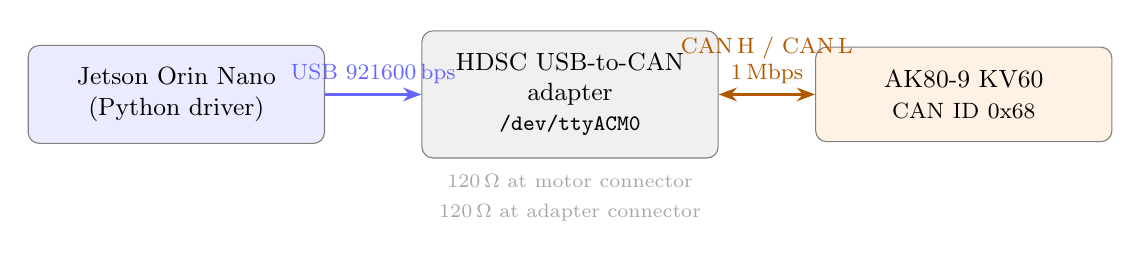
\begin{tikzpicture}[every node/.style={font=\small},
  box/.style={draw=black!50, rounded corners=4pt, inner sep=8pt,
              text width=3.2cm, align=center, minimum height=1.2cm}]

  \node[box, fill=blue!8]  (pc)  at (0,   0) {Jetson Orin Nano\\(Python driver)};
  \node[box, fill=gray!12] (adp) at (5,   0) {HDSC USB-to-CAN\\adapter\\{\footnotesize\texttt{/dev/ttyACM0}}};
  \node[box, fill=orange!10](mot) at (10,  0) {AK80-9 KV60\\{\footnotesize CAN ID 0x68}};

  \draw[-Stealth, thick, blue!60]
    (pc.east)  -- node[above, font=\footnotesize]{USB 921600\,bps} (adp.west);
  \draw[Stealth-Stealth, thick, orange!70!black]
    (adp.east) -- node[above, font=\footnotesize, align=center]{CAN\,H / CAN\,L\\1\,Mbps}   (mot.west);

  % Termination resistors
  \node[font=\scriptsize, text=gray!70] at (5, -1.1) {$120\,\Omega$ at motor connector};
  \node[font=\scriptsize, text=gray!70] at (5, -1.5) {$120\,\Omega$ at adapter connector};
\end{tikzpicture}
\caption{Physical connection chain.  The Python driver writes 30-byte
         HDSC envelope frames to the USB serial port; the adapter
         converts them to CAN 2.0A standard frames on the CAN bus.}
\label{fig:connection}
\end{figure}

\subsection{MIT CAN frame structure}

\subsubsection{Command frame (host $\to$ motor)}

One 8-byte payload packed into standard CAN frame with \texttt{CAN\_ID = ESC\_ID}:

\begin{center}\small
\begin{tabular}{cll}
\toprule
Byte(s) & Contents & Bit layout \\
\midrule
0       & Position upper  & \texttt{q[15:8]} \\
1       & Position lower  & \texttt{q[7:0]} \\
2       & Velocity upper  & \texttt{dq[11:4]} \\
3       & Velocity lower + $K_p$ upper & \texttt{dq[3:0] | Kp[11:8]} \\
4       & $K_p$ lower     & \texttt{Kp[7:0]} \\
5       & $K_d$ upper     & \texttt{Kd[11:4]} \\
6       & $K_d$ lower + $\tau$ upper & \texttt{Kd[3:0] | tau[11:8]} \\
7       & $\tau$ lower    & \texttt{tau[7:0]} \\
\bottomrule
\end{tabular}
\end{center}

Bit-widths: position 16-bit, velocity 12-bit, $K_p$ 12-bit,
$K_d$ 12-bit, $\tau$ 12-bit.  All scaled linearly:
\[
  \texttt{uint} = \left\lfloor
    \frac{x + X_{\max}}{2\,X_{\max}} \cdot (2^{N}-1)
  \right\rfloor
  \quad\text{where }X_{\max} \in \{P_{\max}, V_{\max}, T_{\max}\}
\]

For AK60-6: $P_{\max}=12.5$\,rad, $V_{\max}=45$\,rad/s,
$T_{\max}=15$\,N$\cdot$m.

\subsubsection{Feedback frame (motor $\to$ host)}

The motor replies with \texttt{CAN\_ID = ESC\_ID} (not a separate master
address as with the Damiao motor):

\begin{center}\small
\begin{tabular}{cll}
\toprule
Byte & Contents & Notes \\
\midrule
0 & Motor ESC\_ID    & Redundant with CAN ID \\
1--2 & Position (16-bit) & same scaling as command \\
3--4 & Velocity (upper 8 + lower 4) & 12-bit, $\pm V_{\max}$ \\
4--5 & Torque (lower 4 + 8)         & 12-bit, $\pm T_{\max}$ \\
6   & MOSFET temperature (\textdegree C) & not decoded in current driver \\
7   & Rotor temperature (\textdegree C)  & not decoded in current driver \\
\bottomrule
\end{tabular}
\end{center}

\subsubsection{Special command frames}

Eight-byte payloads with the last byte set to a magic value; the other
seven bytes are \texttt{0xFF}:

\begin{center}\small
\begin{tabular}{ll}
\toprule
Payload (hex) & Function \\
\midrule
\texttt{FF FF FF FF FF FF FF FC} & Enable motor (torque ON) \\
\texttt{FF FF FF FF FF FF FF FD} & Disable motor (torque OFF) \\
\texttt{FF FF FF FF FF FF FF FE} & Set current position as zero \\
\bottomrule
\end{tabular}
\end{center}

% =========================================================================
\section{Two operating modes -- the critical distinction}
\label{sec:modes}
% =========================================================================

The AK80-9 has \textbf{two fundamentally different CAN protocols} that
cannot be mixed.  The mode is stored in flash by R-Link and takes
effect after a power cycle.

\begin{center}\small
\begin{tabular}{p{2.8cm}p{4.8cm}p{4.8cm}}
\toprule
 & \textbf{MIT Mode} & \textbf{Servo Mode (``Periodic Feedback'')} \\
\midrule
R-Link setting  & CAN Mode = \textbf{Inquiry Feedback}
                & CAN Mode = \textbf{Periodic Feedback} \\
CAN frame type  & Standard 2.0A (11-bit ID)
                & Extended 2.0B (29-bit ID) \\
CAN ID scheme   & Command: \texttt{ESC\_ID}\newline
                  Feedback: \texttt{ESC\_ID}
                & Feedback: \texttt{(CMD\_TYPE $\ll$ 8) | ESC\_ID} \\
Frame format    & 8-byte MIT bit-packed
                & VESC/FESC floating-point extended protocol \\
Our driver      & \texttt{cubemars\_bus.py} \textbf{(supported)}
                & \textbf{Not supported} (extended protocol needed) \\
TMotorCANControl& \texttt{MIT\_CAN} class \textbf{(supported)}
                & \texttt{servo\_can} class \\
Feedback timing & On request (reply to MIT poll)
                & Autonomous at configured rate (50\,Hz default) \\
\bottomrule
\end{tabular}
\end{center}

\begin{figure}[ht]
\centering
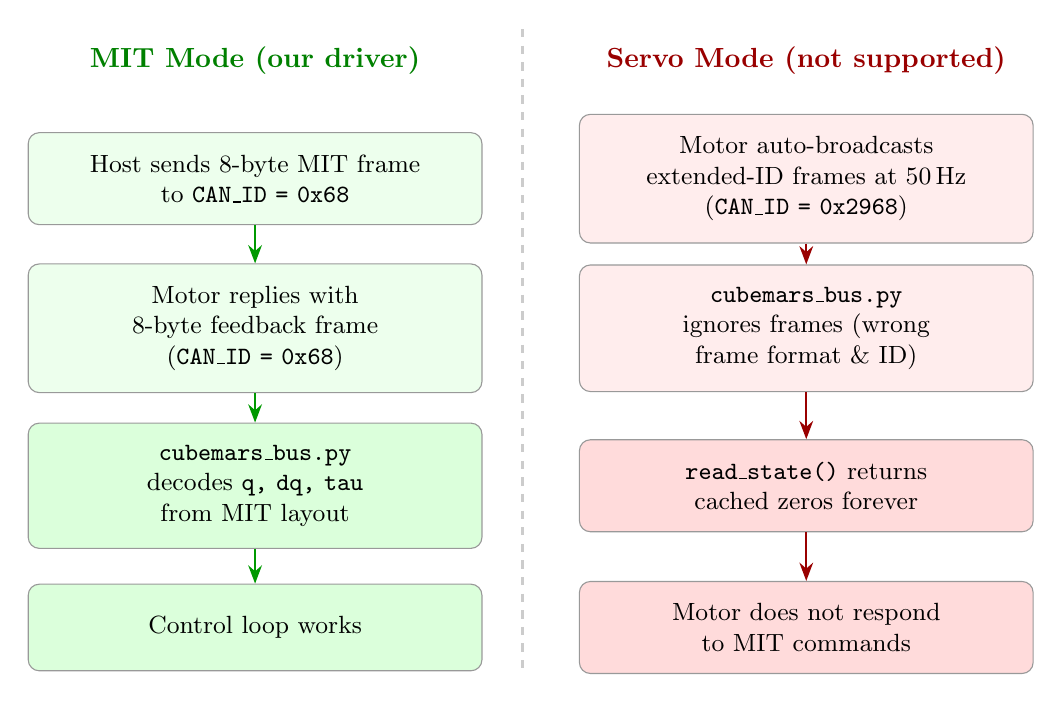
\begin{tikzpicture}[every node/.style={font=\small},
  mbox/.style={draw=black!40, rounded corners=4pt, inner sep=8pt,
               text width=5.2cm, align=center, minimum height=1.1cm}]

  \node[font=\bfseries, text=green!50!black] at (-3.4, 2.0)
    {MIT Mode (our driver)};
  \node[font=\bfseries, text=red!60!black] at ( 3.6, 2.0)
    {Servo Mode (not supported)};
  \draw[dashed, black!20, line width=1pt] (0, 2.4) -- (0, -5.8);

  % MIT path
  \node[mbox, fill=green!7]  (m1) at (-3.4,  0.5)
    {Host sends 8-byte MIT frame\\to \texttt{CAN\_ID = 0x68}};
  \node[mbox, fill=green!7]  (m2) at (-3.4, -1.4)
    {Motor replies with\\8-byte feedback frame\\(\texttt{CAN\_ID = 0x68})};
  \node[mbox, fill=green!14] (m3) at (-3.4, -3.4)
    {\texttt{cubemars\_bus.py}\\decodes \texttt{q, dq, tau}\\from MIT layout};
  \node[mbox, fill=green!14] (m4) at (-3.4, -5.2)
    {Control loop works};
  \draw[-Stealth, green!60!black, thick] (m1) -- (m2);
  \draw[-Stealth, green!60!black, thick] (m2) -- (m3);
  \draw[-Stealth, green!60!black, thick] (m3) -- (m4);

  % Servo path
  \node[mbox, fill=red!7]   (s1) at ( 3.6,  0.5)
    {Motor auto-broadcasts\\extended-ID frames at 50\,Hz\\(\texttt{CAN\_ID = 0x2968})};
  \node[mbox, fill=red!7]   (s2) at ( 3.6, -1.4)
    {\texttt{cubemars\_bus.py}\\ignores frames (wrong\\frame format \& ID)};
  \node[mbox, fill=red!14]  (s3) at ( 3.6, -3.4)
    {\texttt{read\_state()} returns\\cached zeros forever};
  \node[mbox, fill=red!14]  (s4) at ( 3.6, -5.2)
    {Motor does not respond\\to MIT commands};
  \draw[-Stealth, red!60!black, thick] (s1) -- (s2);
  \draw[-Stealth, red!60!black, thick] (s2) -- (s3);
  \draw[-Stealth, red!60!black, thick] (s3) -- (s4);
\end{tikzpicture}
\caption{Divergent behaviour depending on the CAN Mode setting in R-Link.
         The bench motor was found in Servo Mode on 12~May~2026 during
         initial bring-up; see Section~\ref{sec:scan} for the diagnostic.}
\label{fig:modes}
\end{figure}

% =========================================================================
\section{Bench bring-up and the CAN-ID discovery problem}
\label{sec:scan}
% =========================================================================

\subsection{Timeline}

During initial bring-up (12~May~2026) the motor was found to be
broadcasting extended-CAN frames at all times but not responding to MIT
poll commands.  Investigation steps:

\begin{enumerate}
  \item \textbf{R-Link screenshot showed:}
        \texttt{CAN Mode = Periodic Feedback}, \texttt{CAN ID = ID:~4}.
        This placed the motor in \emph{Servo mode}, not MIT mode.
  \item \textbf{MIT poll scan} (\texttt{tests/cubemars/00\_scan\_can\_id.py})
        sent a null MIT frame (\texttt{Kp=Kd=tau=0}) to every CAN ID in
        \texttt{0x01..0x7F}.  Result: 1087 frames received, all from
        extended CAN ID \textbf{\texttt{0x2968}}.
  \item Decoding the extended ID: \texttt{0x2968 = (0x29 << 8) | 0x68}
        where \texttt{0x29} is the VESC/CubeMars servo status command
        type and \texttt{0x68 = 104} is the motor's ESC\_ID.
  \item \textbf{Conclusion:} motor ESC\_ID is \textbf{104 (0x68)}.
        The CAN ID shown in R-Link (\texttt{ID:~4}) was from a previous
        \emph{different} configuration page and was stale.
\end{enumerate}

\subsection{What the extended CAN ID means}

In Servo mode, the motor uses the VESC/FESC extended-CAN protocol:

\begin{center}\small
\begin{tabular}{ll}
\toprule
Field & Value \\
\midrule
Full extended CAN ID (29-bit) & \texttt{0x2968} = 10600 \\
Command type byte (\texttt{cmd = id >> 8}) & \texttt{0x29} = 41 = \texttt{COMM\_GET\_VALUES} \\
Motor ESC\_ID byte (\texttt{mid = id \& 0xFF}) & \texttt{0x68} = 104 \\
Broadcast rate & 50\,Hz (as configured in R-Link) \\
\bottomrule
\end{tabular}
\end{center}

\subsection{Action required}

To use \texttt{cubemars\_bus.py} (MIT mode), open R-Link and apply:

\begin{center}\small
\begin{tabular}{lll}
\toprule
R-Link field & Current value & Required value \\
\midrule
  CAN Mode    & Periodic Feedback & \textbf{Inquiry Feedback} (= MIT mode) \\
CAN Bitrate & 1\,Mbps           & 1\,Mbps (keep) \\
CAN ID      & 4                 & \textbf{104} (or any value -- update \texttt{motor\_config.py}) \\
\bottomrule
\end{tabular}
\end{center}

Click \textbf{Write}, then \textbf{power-cycle the motor} (the mode
change takes effect on reboot, not immediately).

After switching, rerun the scan:
\begin{lstlisting}
python tests/cubemars/00_scan_can_id.py --start 1 --end 127
\end{lstlisting}
You should see one MIT feedback frame at the configured ESC\_ID (not
an extended CAN ID), and the decoder will report valid \texttt{q, dq, tau}.

% =========================================================================
\section{Calibration procedure}
\label{sec:calibration}
% =========================================================================

Unlike the Damiao motor, the AK80-9 has \textbf{no firmware parameter
read API} accessible over CAN.  All calibration steps use R-Link.

\subsection{Required steps (one-time after assembly or firmware flash)}

\begin{enumerate}
  \item \textbf{Motor Identification} -- R-Link spins the motor in both
        directions to measure winding resistance, inductance, and
        back-EMF constant.  Motor must be unloaded (disconnected from
        gearbox output if possible, or at least free to spin).
  \item \textbf{Encoder Identification} -- R-Link samples the encoder
        at many positions and builds a lookup table for pole-pair offset.
        Must be done immediately after Motor Identification.
  \item \textbf{Write Parameters} -- Click \emph{Write} in R-Link to
        flash the identified values.  Save \texttt{.AppParams} and
        \texttt{.McParams} files as backups.
\end{enumerate}

\noindent Re-calibrate after:
\begin{itemize}
  \item Swapping any two of the three motor phase wires.
  \item Replacing the motor or gearbox.
  \item Flashing new firmware.
\end{itemize}

\subsection{Software zero position}

\texttt{cubemars\_bus.py} supports software-latching of the current
angle as $0\,\mathrm{rad}$ via the special frame
\texttt{[FF FF FF FF FF FF FF FE]}:

\begin{lstlisting}
with open_cubemars_bus(set_zero=True) as bus:
    # motor's current angle is now 0 rad for this session
    bus.write("goal_position", {"j1": 1.0}, kp=30, kd=1.0)
\end{lstlisting}

This is volatile -- it resets on power-cycle.

% =========================================================================
\section{MIT control modes}
\label{sec:control}
% =========================================================================

The five MIT parameters give access to three practical control modes
by choosing which are nonzero:

\begin{center}\small
\begin{tabular}{lllll}
\toprule
Mode & $K_p$ & $K_d$ & $q_{\text{des}}$ & $\dot{q}_{\text{des}}$ \\
\midrule
Position hold     & $>0$  & $>0$  & target rad & 0 \\
Velocity tracking & 0     & $>0$  & 0          & target rad/s \\
Open-loop torque  & 0     & 0     & 0          & 0 \\
\bottomrule
\end{tabular}
\end{center}

\textbf{Warning:} never command $K_p > 0$, $K_d = 0$ in position mode.
Without damping the motor oscillates or runs away.

\subsection{Recommended gains for AK60-6}

\begin{center}\small
\begin{tabular}{llll}
\toprule
Task & $K_p$ & $K_d$ & Notes \\
\midrule
Stiff position hold  & 80--150 & 2.0--4.0  & Heavy load; increase $K_d$ first \\
Compliant hold       & 30--60  & 1.0--2.0  & Lighter load or back-drivable \\
Impedance (teaching) & 0--10   & 0.3--0.8  & Very compliant; record demos \\
Velocity tracking    & 0       & 1.0--3.0  & $K_p=0$ mandatory \\
Torque (open-loop)   & 0       & 0         & Max 1\,N$\cdot$m unloaded (T\_MAX=15\,N$\cdot$m) \\
\bottomrule
\end{tabular}
\end{center}

\subsection{Impedance / kinesthetic teaching}

To make the motor back-drivable for demonstration recording:

\begin{lstlisting}
with open_cubemars_bus() as bus:
    while recording:
        q, dq, tau = bus.read_state()["j1"]
        bus.write("goal_position", {"j1": q},   # spring at current pos
                  kp=5.0, kd=0.5)               # very soft
        record(t, q, dq, tau)
\end{lstlisting}

Replay with higher stiffness:
\begin{lstlisting}
bus.write("goal_position", {"j1": target_q}, kp=60, kd=2.0)
\end{lstlisting}

% =========================================================================
\section{HDSC USB-to-CAN adapter -- frame envelope}
\label{sec:hdsc}
% =========================================================================

The Python driver does not use a SocketCAN or PCAN interface; it writes
a vendor-specific 30-byte serial envelope directly to the HDSC adapter.
The adapter converts this internally to a CAN 2.0A standard frame.

\subsubsection{Transmit envelope (30 bytes, host $\to$ adapter)}

\begin{center}\footnotesize
\begin{tabular}{ccp{7cm}}
\toprule
Bytes & Value (hex) & Meaning \\
\midrule
0     & \texttt{55}          & Start-of-frame \\
1     & \texttt{AA}          & Start-of-frame \\
2     & \texttt{1E}          & Frame length = 30 \\
3     & \texttt{03}          & Command type (send CAN frame) \\
4--8  & \texttt{01 00 00 00 0A} & Fixed header fields \\
9--12 & \texttt{00 00 00 00} & Reserved \\
13    & \texttt{CAN\_ID[7:0]} & CAN ID lower byte = ESC\_ID \\
14    & \texttt{CAN\_ID[10:8]} & CAN ID upper bits (for IDs $\le$0x7FF always 0) \\
15--20& \texttt{00 00 08 00 00 00} & Fixed (DLC=8) \\
21--28& payload & 8-byte MIT payload \\
29    & (computed)   & Unused / padding \\
\bottomrule
\end{tabular}
\end{center}

\subsubsection{Receive frame (16 bytes, adapter $\to$ host)}

\begin{center}\footnotesize
\begin{tabular}{ccp{6cm}}
\toprule
Bytes & Value (hex) & Meaning \\
\midrule
0     & \texttt{AA}          & Start byte \\
1     & \texttt{11}          & Command type (motor feedback) \\
2     & \texttt{08}          & DLC = 8 \\
3--6  & CAN ID (4-byte LE)   & For MIT: CAN\_ID = ESC\_ID \\
7--14 & payload              & 8-byte MIT feedback payload \\
15    & \texttt{55}          & End byte \\
\bottomrule
\end{tabular}
\end{center}

\noindent The driver scans for \texttt{0xAA} start / \texttt{0x55} end
markers (16 bytes apart) and discards partial frames.

\paragraph{Servo-mode extended CAN ID.}
When the motor is in Servo~Mode, the feedback CAN ID is 29-bit
(\texttt{0x2968} for our motor), but the HDSC adapter still delivers
it in the 4-byte little-endian field (bytes~3--6).  The driver compares
against the configured ESC\_ID (\texttt{0x68}) and these 4 bytes will
never match (they decode to \texttt{0x00002968} = 10600), so \emph{all
servo-mode frames are silently discarded}.  This is the root cause of
the ``all zeros'' symptom.

% =========================================================================
\section{Python driver architecture}
\label{sec:driver}
% =========================================================================

\begin{center}\small
\begin{tabular}{ll}
\toprule
File & Role \\
\midrule
\texttt{src/motor\_config.py}   & Declarative config dataclasses + \texttt{DEFAULT\_CUBEMARS\_BENCH\_CONFIG} \\
\texttt{src/cubemars\_bus.py}  & Self-contained MIT bus driver (\texttt{CubemarsMotorsBus}) \\
\texttt{src/\_common.py}       & \texttt{open\_cubemars\_bus()} context-manager helper \\
\texttt{tests/cubemars/}       & Numbered test scripts 00--07 \\
\bottomrule
\end{tabular}
\end{center}

\subsection{Context-manager idiom (all tests)}

\begin{lstlisting}
from _common import open_cubemars_bus

with open_cubemars_bus(set_zero=True) as bus:
    bus.write("goal_position", {"j1": 1.57}, kp=30, kd=1.0)
    q, dq, tau = bus.read_state()["j1"]
\end{lstlisting}

\subsection{Test script inventory}

\begin{center}\small
\begin{tabular}{lp{9cm}}
\toprule
Script & Purpose \\
\midrule
\texttt{00\_scan\_can\_id.py}          & Sweep IDs 0x01--0x7F, identify motor; also detects Servo Mode\\
\texttt{01\_check\_connection.py}      & Poll 5 feedback frames, confirm non-zero \\
\texttt{02\_mit\_position.py}          & MIT position hold, step through angles \\
\texttt{03\_mit\_velocity.py}          & MIT velocity tracking \\
\texttt{04\_mit\_torque.py}            & Open-loop torque ($\le$1\,N$\cdot$m unloaded) \\
\texttt{05\_kinesthetic\_record.py}    & Hand-guide + save \texttt{demo\_trajectory\_ak80.csv} \\
\texttt{06\_replay\_trajectory.py}     & Replay the recorded CSV \\
\texttt{07\_impedance\_spring\_return.py} & Soft spring anchored at zero \\
\bottomrule
\end{tabular}
\end{center}

% =========================================================================
\section{Known issues and gotchas}
\label{sec:gotchas}
% =========================================================================

\begin{enumerate}

\item \textbf{[CURRENT ISSUE] Motor is in Servo Mode.}
  The motor auto-broadcasts extended-CAN status frames at 50\,Hz
  (CAN~ID \texttt{0x2968}, cmd \texttt{0x29}, motor ID \texttt{0x68} = 104).
  \texttt{cubemars\_bus.py} speaks MIT only (standard CAN).  All
  feedback is silently discarded; \texttt{read\_state()} returns zeros.
  \textbf{Fix:} R-Link $\to$ CAN Mode = \textbf{Inquiry Feedback} $\to$ Write
  $\to$ power-cycle.
  feedback frame is 104 (\texttt{0x68}).  \texttt{motor\_config.py}
  has been corrected to \texttt{can\_id=0x68}.

\item \textbf{Model is AK60-6 V3.0 KV80, not AK80-9.}
  R-Link hardware/software version string \texttt{AK60\_6V} /
  \texttt{AK60\_6\_SE\_V3} confirmed on 12~May~2026.  All MIT limits
  updated to AK60-6 values:
  \texttt{CUBEMARS\_LIMITS["AK60-6"] = [12.5, 45.0, 15.0]}.

\item \textbf{Never Kd = 0 in position mode.}
  Same rule as Damiao MIT mode: $K_d = 0$ with $K_p > 0$ removes all
  damping and causes oscillation or runaway.

\item \textbf{Calibration required before first use.}
  Run Motor Identification + Encoder Identification in R-Link with the
  motor unloaded.  Write parameters.  Re-run if any phase wire is swapped.

\item \textbf{No mode switch over CAN.}
  The MIT / Servo mode switch is a flash-stored setting only changeable
  via R-Link + power-cycle.  It cannot be commanded over CAN at runtime.

\item \textbf{Peak current caution.}
  The motor allows up to 30\,A peak.  When testing open-loop torque
  (\texttt{04\_mit\_torque.py}), keep $\tau_{\text{ff}} \le 1$\,N$\cdot$m
  when unloaded to avoid damaging a current-limited bench supply.

\end{enumerate}

% =========================================================================
\section{TMotorCANControl reference library}
\label{sec:tmotor}
% =========================================================================

The \texttt{TMotorCANControl/} directory contains the
\href{https://github.com/neurobionics/TMotorCANControl}{neurobionics/TMotorCANControl}
open-source library, included as a vendored reference.  It implements
the same MIT CAN protocol for T-Motor / CubeMars actuators using
\textbf{SocketCAN} (Linux \texttt{can0} interface via \texttt{python-can}).

\subsection{How it differs from our driver}

\begin{center}\small
\begin{tabular}{lll}
\toprule
Aspect & \texttt{cubemars\_bus.py} (ours) & TMotorCANControl \\
\midrule
CAN interface & HDSC USB-to-CAN serial (\texttt{/dev/ttyACM0}) &
               SocketCAN (\texttt{can0}, \texttt{slcan}, etc.) \\
Dependency & \texttt{pyserial} only & \texttt{python-can}, SocketCAN kernel module \\
Jetson setup & Plug-in USB adapter, no kernel config & Requires \texttt{ip link set can0 up} \\
MIT protocol & Identical bit-packing & Identical bit-packing \\
Servo mode  & Not supported & Supported via \texttt{servo\_can} class \\
API style   & LeRobot-style \texttt{read}/\texttt{write} & Iterator / context manager \\
\bottomrule
\end{tabular}
\end{center}

\subsection{Using TMotorCANControl (reference, not our primary path)}

If you want to switch to SocketCAN on the Jetson (for lower latency or
multi-motor daisy-chaining without the HDSC adapter):

\begin{lstlisting}[language=bash, numbers=none]
# Bring up SocketCAN interface (HDSC adapter exposes slcan):
sudo slcand -o -c -s8 /dev/ttyACM0 can0
sudo ip link set can0 up type can bitrate 1000000

# Then use TMotorCANControl:
from TMotorCANControl.mit_can import TMotorManager_mit_can
with TMotorManager_mit_can(motor_type="AK80-9", device="can0",
                           motor_ID=104) as m:
    m.set_zero_position()
    m.update()
    print(m.position, m.velocity, m.torque)
\end{lstlisting}

\textbf{Note:} the HDSC adapter firmware does not natively speak
\texttt{slcan}, so the above may require the \texttt{slcan} TTY line
discipline.  Our \texttt{cubemars\_bus.py} avoids this by writing the
HDSC proprietary 30-byte envelope directly, which is more reliable on
Jetson without kernel module setup.

% =========================================================================
\section{Quick-start checklist}
\label{sec:checklist}
% =========================================================================

\begin{enumerate}
  \item Power on motor (18--52\,V; bench uses 48\,V).
  \item Connect HDSC USB-to-CAN adapter to Jetson USB port.
  \item Verify \texttt{ls /dev/ttyACM0} exists.
  \item \textbf{Ensure motor is in MIT mode} (R-Link $\to$ CAN Mode = MIT,
        Write, power-cycle).
  \item Run scan to confirm CAN ID:
\begin{lstlisting}[numbers=none]
conda activate actuators
cd tests/cubemars
python 00_scan_can_id.py
\end{lstlisting}
  \item Expected: one MIT feedback frame at \texttt{0x68} (104) with valid
        \texttt{q, dq, tau}.
  \item If scan shows extended-ID \texttt{0x2968}: motor is still in Servo
        Mode.  Return to step~4.
  \item Run connection check:
\begin{lstlisting}[numbers=none]
python 01_check_connection.py
\end{lstlisting}
  \item Proceed with higher test scripts (\texttt{02}--\texttt{07}).
\end{enumerate}

\end{document}
